\documentclass[a4paper,12pt]{article} % тип документа

% report, book
\usepackage[english,russian]{babel} %локализация и переносы
\usepackage{float}

%Вставка картинок
\usepackage{wrapfig}
\usepackage{graphicx}
\graphicspath{{pictures/}}
\DeclareGraphicsExtensions{.pdf,.png,.jpg}

%Графики
\usepackage{multirow}
\usepackage{pgfplots}
\pgfplotsset{compat=1.9}

%Математика
\usepackage{amsmath, amsfonts, amssymb, amsthm, mathtools}
\usepackage{physics}
% Рисунки
\usepackage{graphicx}
\usepackage{wrapfig}
\usepackage{mathtext}
\usepackage[left=2cm,right=2cm,
    top=2cm,bottom=2cm,bindingoffset=0cm]{geometry}
\usepackage{multirow}
\usepackage{pgfplots}
\usepackage{hyperref}
\usepackage[rgb]{xcolor}
\hypersetup{				% Гиперссылки
    colorlinks=true,       	% false: ссылки в рамках
	urlcolor=blue          % на URL
}

%  Русский язык

\usepackage[T2A]{fontenc}			% кодировка
\usepackage[utf8]{inputenc}			% кодировка исходного текста
\usepackage[english,russian]{babel}	% локализация и переносы


% Математика
\usepackage{amsmath,amsfonts,amssymb,amsthm,mathtools} 


\usepackage{wasysym}

\author{Павловский Кирилл. Завьялов Артем. Б01-207}
\title{\textbf{Лабораторная работа. 1.3.4\\ Исследование стационарного потока жидкости в трубе}}
\date{}
\begin{document}
\maketitle
\thispagestyle{empty}
\newpage

\subsection*{Аннотация}
В данной работе измеряется скорость течения по методам Пито и Вентури, а также сравниваются результаты со скоростью, определенной по расходу воды. Для этого в работе используется расходомерная установка.

\subsection*{Теоретические сведения}
\begin{figure} [h]
\centering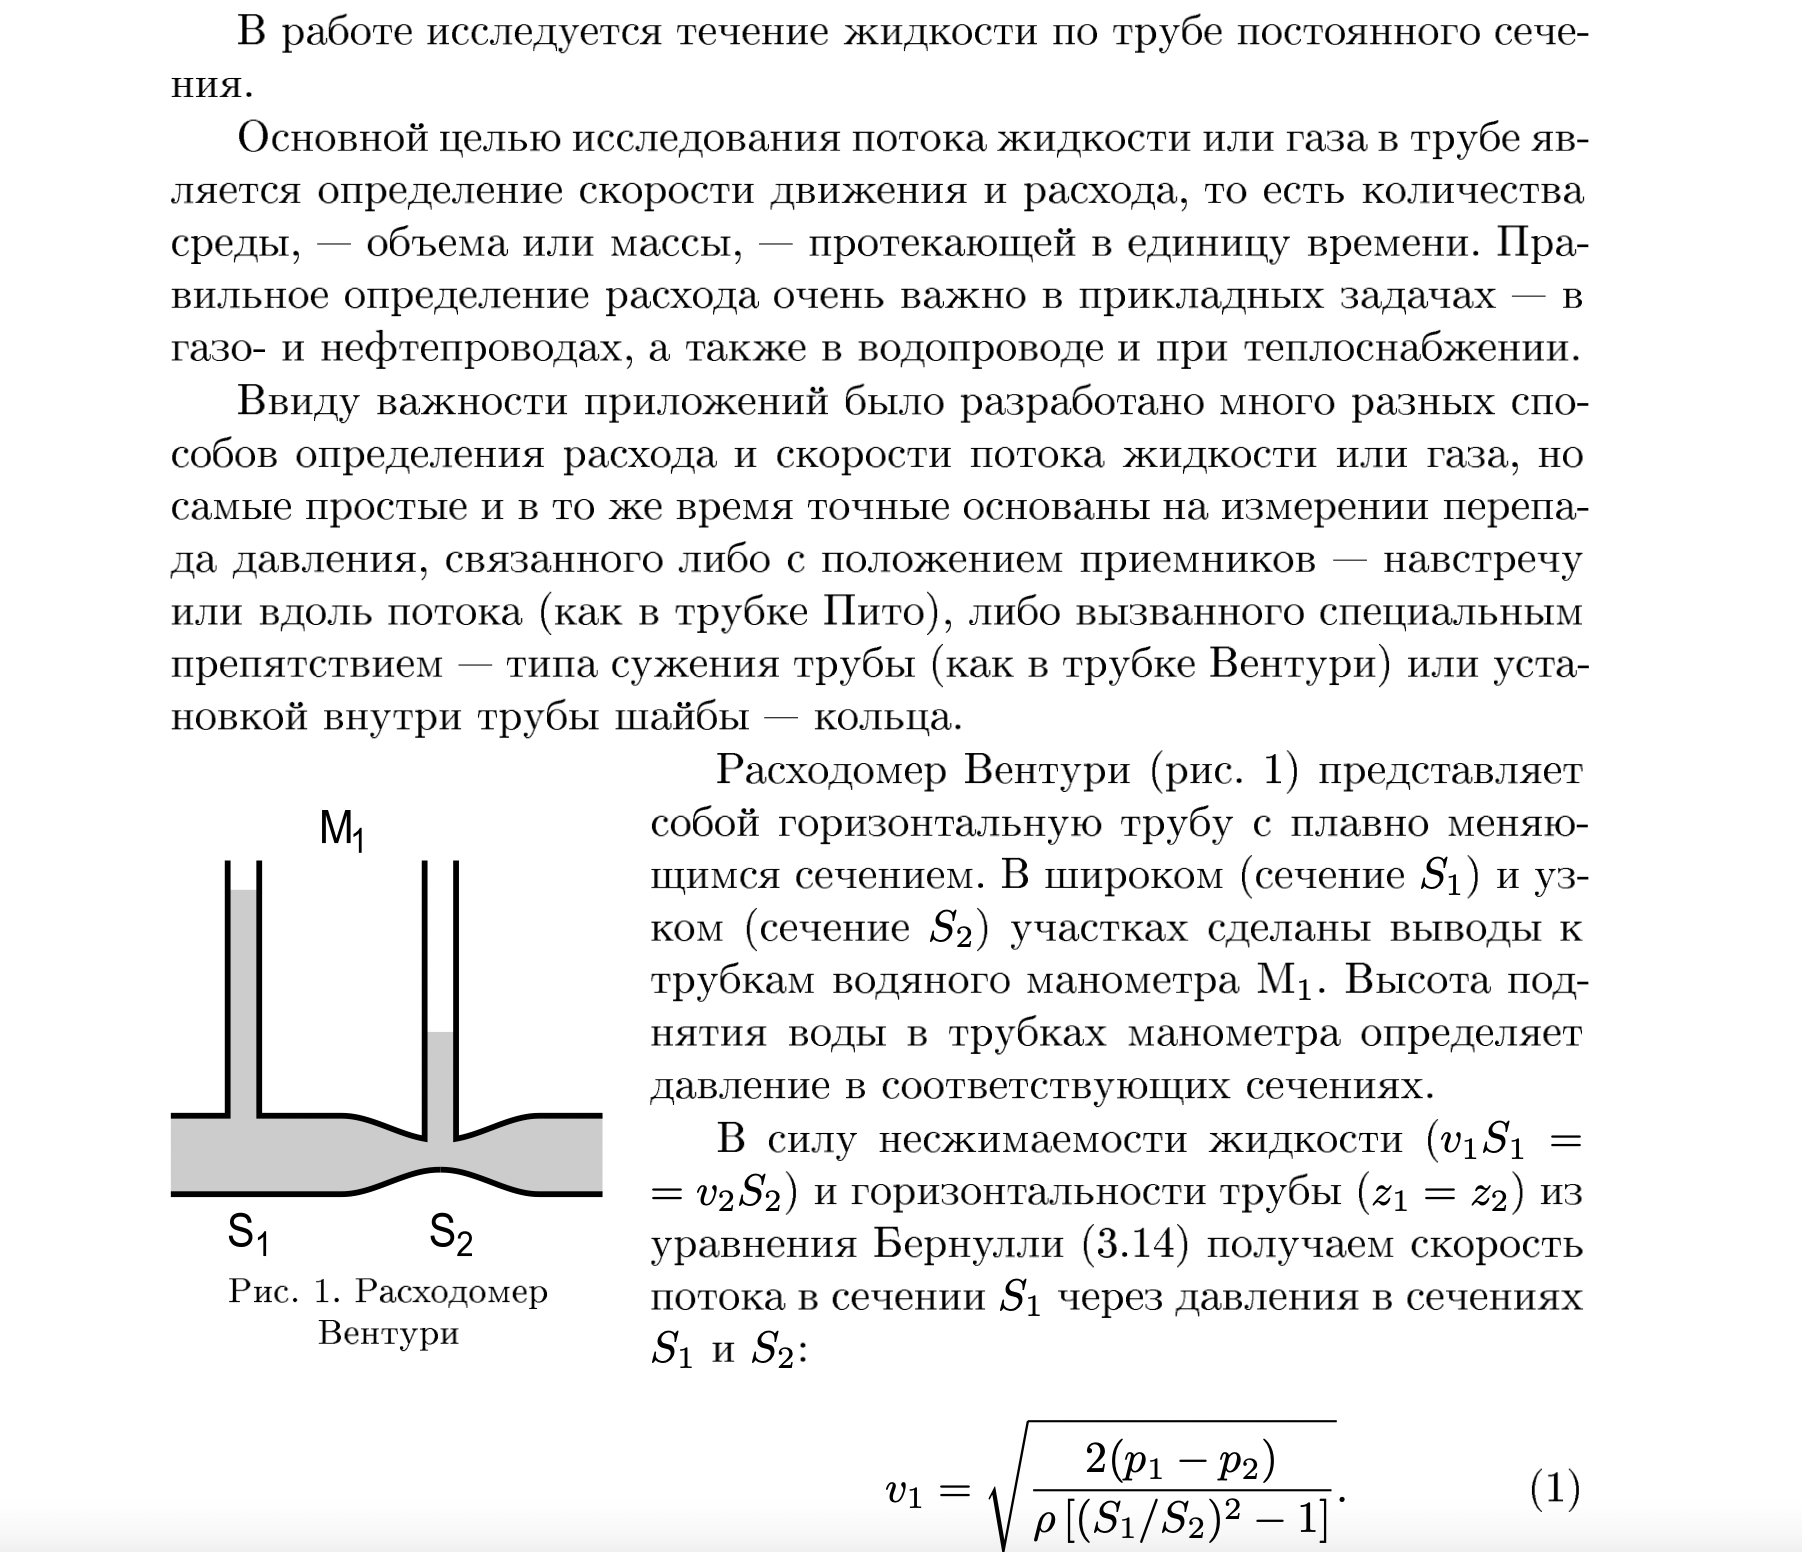
\includegraphics[scale = 0.5]{Snimok_Ekrana_2023-06-11_V_13_40_21.png}
\end{figure}

\begin{figure} [h]
\centering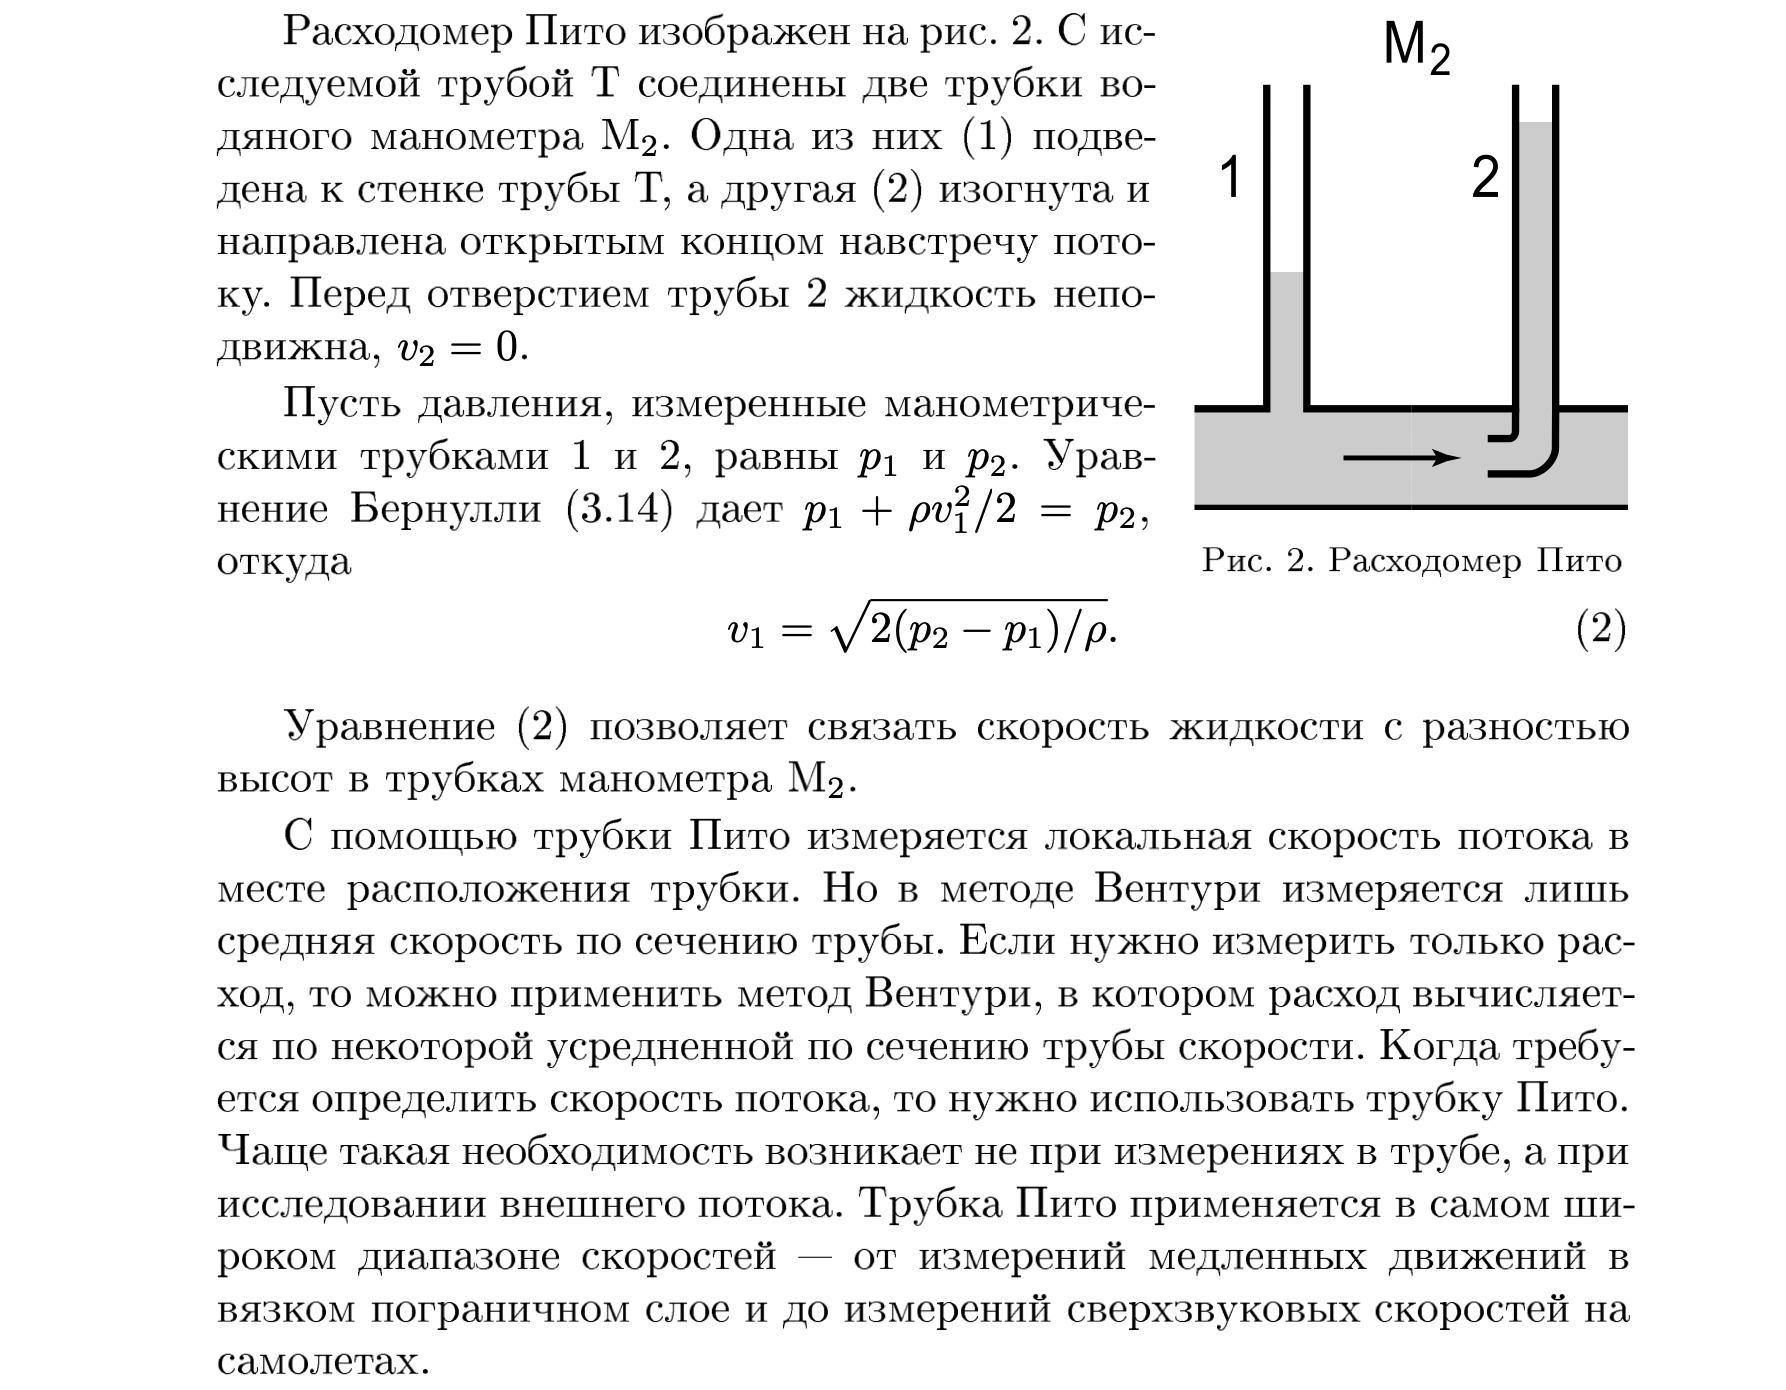
\includegraphics[scale = 0.5]{Snimok_Ekrana_2023-06-11_V_13_41_45.png}
\end{figure}

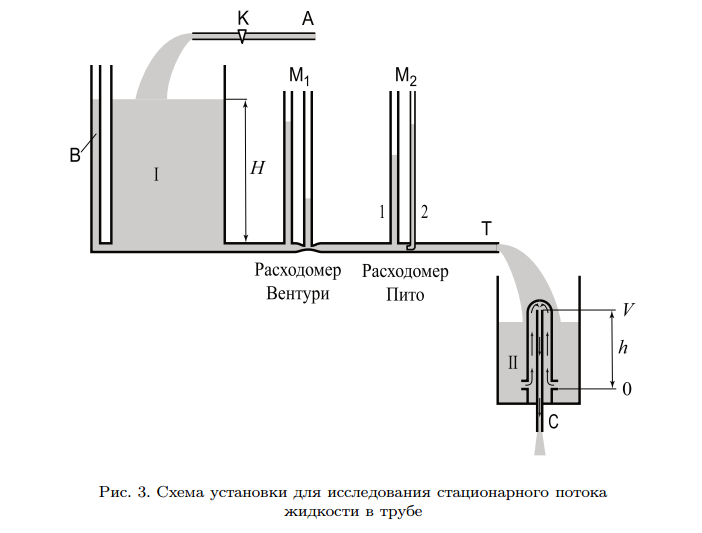
\includegraphics[width=\textwidth]{facility.png}
\\
I - цилиндрический резервуар\\
II - приёмный резервуар известного объёма\\
А - водопроводная труба\\
Т - труба с исследуемой водой\\
К - кран для регулировки поступающей воды\\
	\vspace{0.2cm}
С - сифон, автоматически выливающий воду по дистижении ей уровня h\\

Скорость течения, усредненную по сечению трубы, можно определить по расходу, который находится по измеренному времени наполнения резервуара II, объем которого задан. С другой стороны, скорость
может быть рассчитана по показаниям манометров. Сопоставление этих скоростей со скоростью, определенной по расходу, позволяет сделать вывод о применимости уравнения Бернулли, роли вязкости, которая, в частности, приводит к изменению скорости поперек потока.
 Для количественной оценки роли вязкости необходимо проделать следующий эксперимент.Установив уровень жидкости в резервуаре I на определенной высоте $z{}_1{}$ измерить скорость течения жидкости по трубе Т с помощью приемного резервуара II (в силу несжимаемости жидкости ее скорость на входе в трубу Т и на выходе из нее одинакова). По измеренному значению
скорости по формуле Торричелли рассчитать ту высоту $z{}_2{}$, при которой жидкость вытекала бы с этой же скоростью в отсутствие вязкости\\
Разность $z{}_1{} - z{}_2{}$ характеризует потери на внутреннее трение в жидкости, причем можно считать, что эти потери происходят только в трубе Т, так как скорость жидкости в резервуаре I существенно меньше.
Влияние вязкости изменяет показания манометра Вентури $\triangle h$ на
величину, которую можно оценить, умножив разность $z{}_1{} - z{}_2{}$ на отношение расстояния между входами манометра $\triangle l$ ко всей длине трубы $L$. При условии
\begin{center}
$\triangle h \geq(z{}_1{} - z{}_2{})\frac {\triangle l}{L}$
\end{center}
неидеальностью жидкости в пределах манометра М можно пренебречь.
В противном случае ($\triangle h$ сравнимо с $z{}_1{} - z{}_2{})\frac {\triangle l}{L}$
 в уравнении для расходомера Вентури из
$p{}_1{} - p{}_2{}$ необходимо вычесть $\triangle z\frac {\triangle l}{L}\rho g$\\
Это же верно и для расходомера Пито. Кроме этого, для трубки Пито слеудет сделать оценку поправки к его показаниям, вызванную конечностью размеров вставленной в поток частью изогнутой трубки 2.
При измерениях очень важно обеспечить стационарность течения жидкости. Это достигается тем, что уровень воды в резервуаре I при каждом измерении  помощью крана К должен поддерживаться на одной и той же высоте Н.

\section{Ход работы}

Параметры установки:\\
$L = (22.2 \pm 0,1) $cм\\
$D_{v} = 1 $cм(большой диаметр трубки Вентури)\\
Отсюда находим площадь этой трубки
$S_{1} = 0.785 \text{cм}^2$\\
$d_{v} = 0.6 $cм(малый диаметр трубки Вентури)\\
Отсюда получим ее площадь
$S_{2} = 0.283 \text{cм}^2$\\
$\Delta l = 0.02 $м(расстояние между сечениями трубки Вентури)\\
$D_{p} = 1 $cм(диаметр трубки Пито)\\
$V = (276 \pm 4) \cdot 10^{-5} \text{м}^3$(обьем, который заполняет жидкость в резервуаре II) \\
Измерим длину и ширину заполняемого резервуара. l = $20 \pm 0.1$cм и h = $19.7 \pm 0.1$cм. Отсюда находим его площадь:
S = 394$\text{см}^2$\\
h = ($7 \pm 0,1$)см (высота заполнения резервуара)\\

Проводим измерения времени заполнения резервуара II в зависимости от высоты уровня жидкости Н в резервуаре I. Для каждой фиксированной высоты H проводим 2 измерения. Результаты записываем в таблицу (1)\\

\begin{table}[h!]
\begin{center}
    \begin{tabular}{|c|c|c|c|c|}
    \hline
    Н, cm & t_{1}, c & t_{2}, c & \Delta h_{v}, cm & \Delta h_{p}, cm\\ \hline
    79 & 46.98 & 47.32 & 19.6 & 4.5 \\ \hline
    69 & 50.78 & 51.17 & 16.5 & 4.4 \\ \hline
    59 & 57.06 & 56.41 & 13.9 & 3.5  \\ \hline
    50 & 60.21 & 61.77 & 12.0 & 2.9 \\ \hline
    40 & 66.01 & 68.67 & 9.6 & 2.2 \\ \hline
    30 & 77.8 & 77.12 & 7.1 & 1.7 \\ \hline
    23 & 90.3 & 92.72 & 5.4 & 1.2 \\ \hline
    \end{tabular}
    \label{sensitivity}
    \caption {Результаты измерения показаний манометров}
\end{center}
\end{table}

По среднему времени заполнения резервуара водой вычислим скорость течения воды по расходу $v_p=\frac {V}{tS_1}$. Оценим погрешность определения скорости по формуле $(\frac {\sigma_v}{v})^2=(\frac {\sigma_t}{t})^2+(\frac {\sigma_V}{V})^2$, где ${\sigma_t} = \sqrt{\frac{1}{n(n-1)}\sum_{i=1}^n (t_i-\langle x \rangle)^2\quad}$ - относительная погрешность.Относительную погрешность скорости будем вычислять как сумму относительных погрешностей объема и времени. Также посчитаем значение $h_{theor} = v^2 / (2g)$ -высота, расчитанная по формуле Торричелли. Результаты занесём в таблицу (2)\\

\begin{table}[h]
    \begin{center}
    \begin{tabular}{|c|c|c|c|c|c|c|c|}
    \hline
 $H, m$ & $t, c$ & $\sigma_t, c$ & $v, m/c$ & $v^2, m^2/c^2$ & $\sigma_v , m/c$ & $\sigma_{v^{2}}, m^2/c^2 $ & $h_{theor}, m$\\ \hline 
 0.79 & 47.2 & 0.17 & 0.75 & 0.56 & 0.02 & 0.04 & 0.029\\ \hline
 0.69 & 51.0 & 0.20 & 0.69 & 0.48 & 0.02 & 0.04 & 0.024\\ \hline
 0.59 & 56.7 & 0.33 & 0.62 & 0.38 & 0.02 & 0.04 & 0.019\\ \hline
 0.50 & 61.0 & 0.78 & 0.58 & 0.34 & 0,02 & 0.04 & 0.0174\\ \hline
 0.40 & 67.3 & 1.33 & 0.53 & 0.28 & 0.02 & 0.04 & 0.014\\ \hline
 0.30 & 77.5 & 0.34 & 0.45 & 0.20 & 0.02 & 0.04 & 0.010\\ \hline
 0.23 & 91.5 & 1.21 & 0.39 & 0.15 & 0.02 & 0.04 & 0.008\\ \hline
 \hline
\end{tabular}
\caption{Расчёт скорости течения по расходу, его погрешность}
\end{center}
\end{table}
Исходя из этих результатов посторим график зависимости квадрата скорости от уровня воды в баке и график квадрата скорости от высоты, расчитанной по формуле Торричелли(график 1).

\begin{figure}[h!]
	\begin{center}
		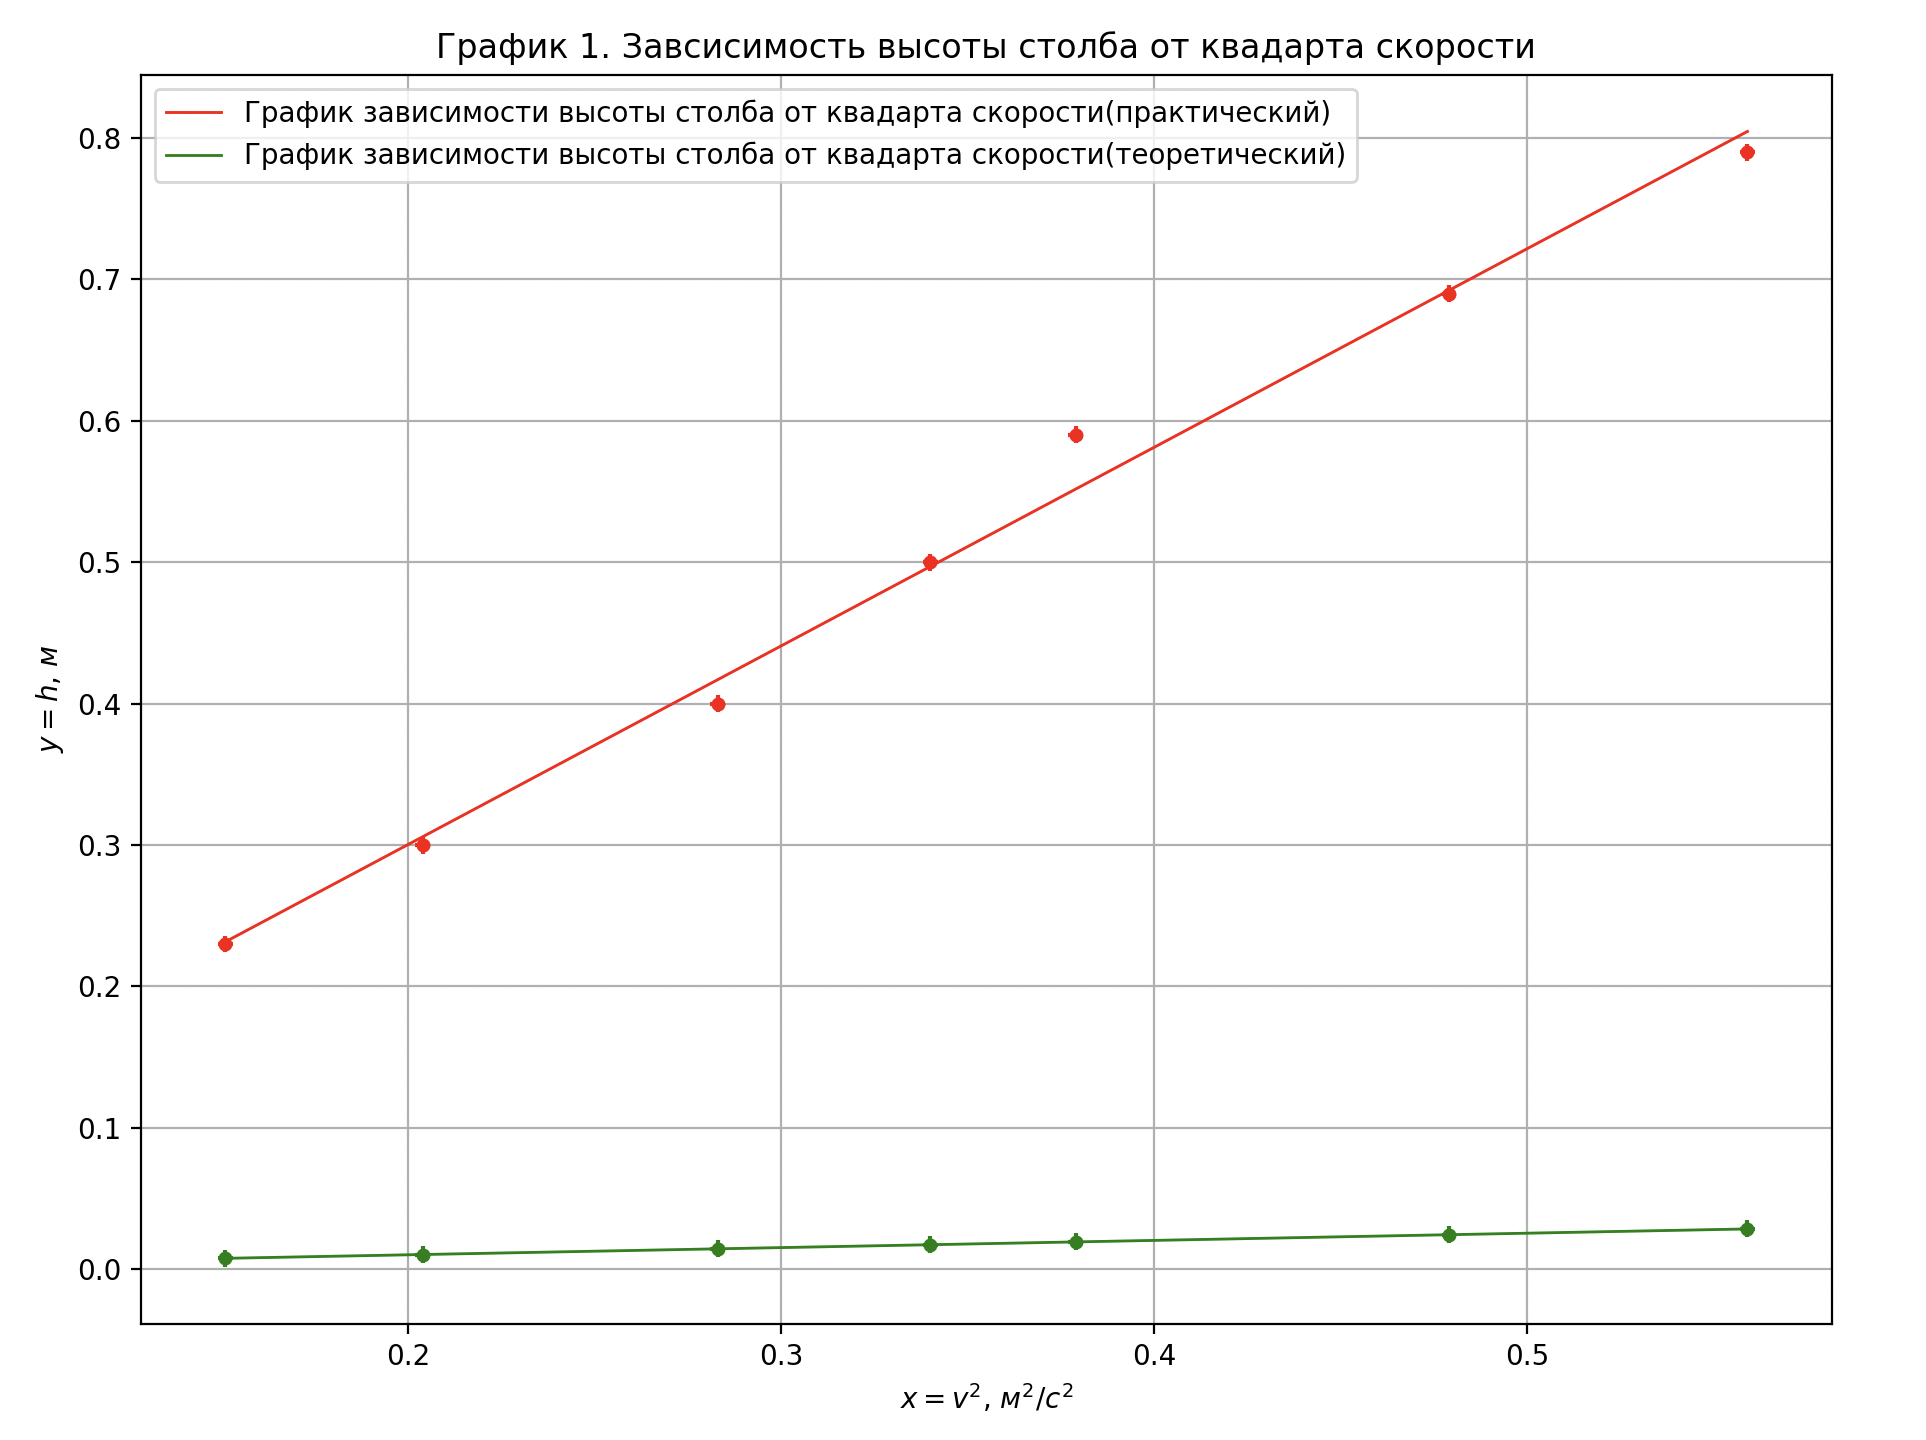
\includegraphics[width=18cm]{Snimok_Ekrana_2023-06-11_V_16_55_59.png}
	\end{center}
	\caption{Зависимость h(v^2)}
	\label{ust}
\end{figure}

Из графика видно, что практический и теоретический результат сильно сотличаются друг от друга. Это связано с тем, что мы не учитывали вязкость воды при расчете предполагаемой высоты столба. То есть, жидкость неидельана.

Теперь по формулам расходомеров Вентури и Пито вычислим скорость течения без учета потерь и с учетом потерь. 

В уравнении для расходомера Вентури из
$p{}_1{} - p{}_2{}$ необходимо вычесть $\triangle z\frac {\triangle l}{L}\rho g$\\
Где $\Delta z = z_{1} - z_{2}$, $z_{1}$ - уровень высоты жидкости в резервуаре I, $z_{2}$ - высота, измеренная по формуле Торричелли.\\ 
Для расходомера Пито проведём следующую оценку\\
Скорость жидкости в центре трубы по формуле Пуазейля:
\begin{center}
$v_0 =\frac{1}{4\nu}\frac{\triangle P}{L}(R^2)$
\end{center}
Скорость жидкости у края трубки расходомера Пито:\\
\begin{center}
$v(r) =\frac{1}{4\nu}\frac{\triangle P}{L}(R^2-r^2)$
\end{center}
Средняя скорость в трубке Пито:\\
\begin{center}
$v_P =\frac{1}{4\nu}\frac{\triangle P}{L}(R^2-\frac{r^2}{2})$
\end{center}
Тогда\\
\begin{center}
$\frac{1}{4\nu}\frac{\triangle P}{L} =\frac{v_0}{R^2}$
\end{center}
Окончательно средняя скорость воды в трубе:\\
\begin{center}
$v_0 =\frac{v_P R^2}{R^2-\frac{r^2}{2}}$
\end{center}

Результаты измерений представлены в таблице (3)

\begin{table}[H]
\begin{center}
    \begin{tabular}{|c|c|c|c|c|}
    \hline
    v_{расход}, m/c & v_{v}, m/c & v_{p}, m/c & v*_{v}, m/c & v*_{p}, m/c\\ \hline
    0.75 & 0.76 & 0.94 & 0.88 & 1.15 \\ \hline
    0.69 & 0.69 & 0.93 & 0.81 & 1.13 \\ \hline
    0.62 & 0.64 & 0.83 & 0.75 & 1.01  \\ \hline
    0.58 & 0.59 & 0.75 & 0.69 & 0.92 \\ \hline
    0.53 & 0.53 & 0.66 & 0.62 & 0.80 \\ \hline
    0.45 & 0.46 & 0.58 & 0.53 & 0.70 \\ \hline
    0.39 & 0.40 & 0.49 & 0.47 & 0.59 \\ \hline
    \end{tabular}
    \label{sensitivity}
    \caption {Значения скоростей, расчитанных при помощи расходомеров}
\end{center}
\end{table}

Представим полученные скорости на одном графике в зависимости от V_{расхода}

\begin{figure}[H]
	\begin{center}
		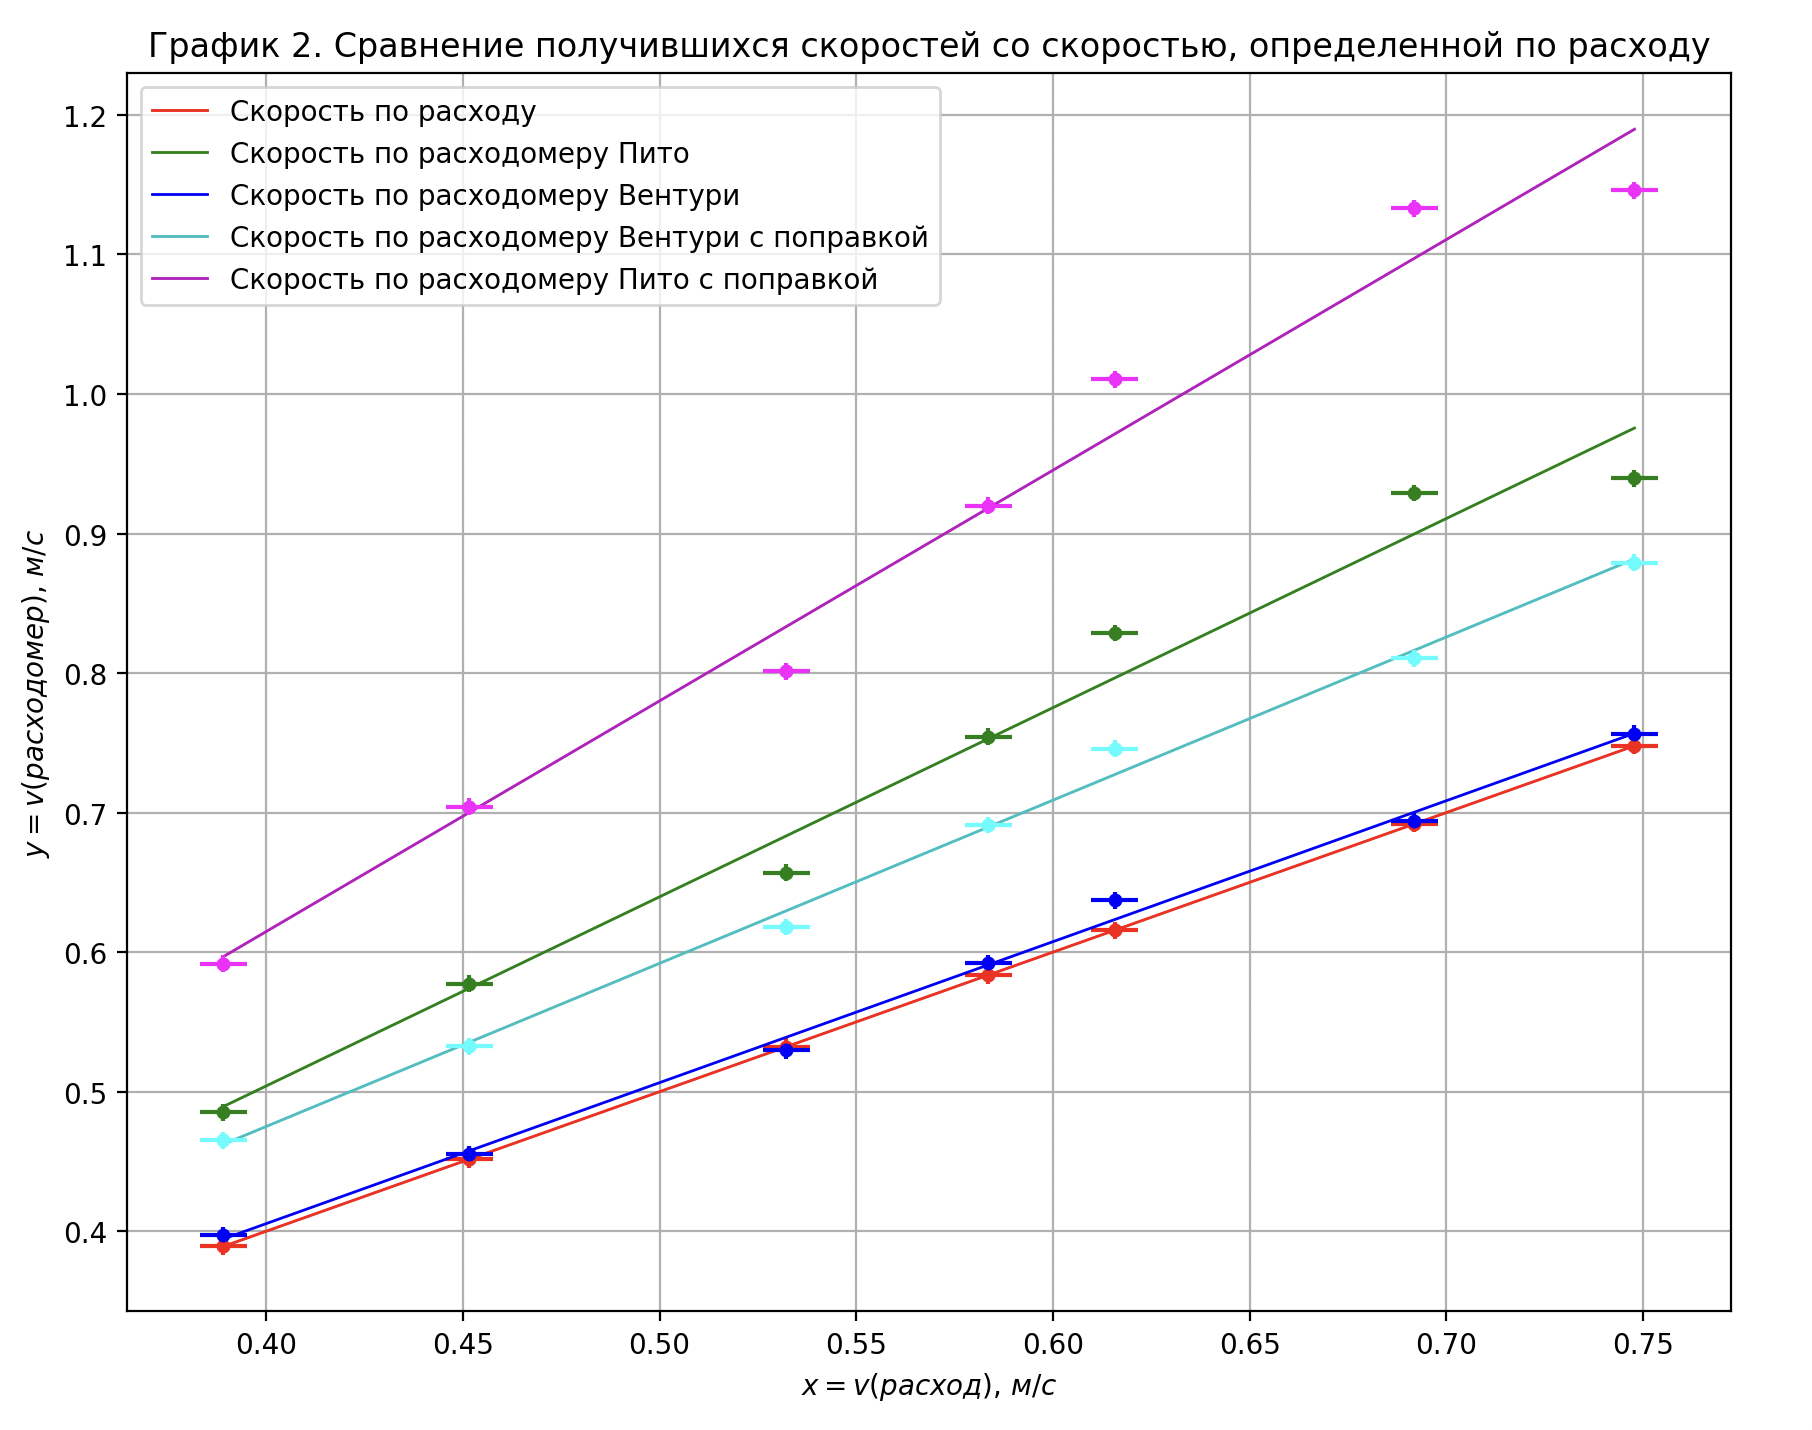
\includegraphics[width=18cm]{Snimok_Ekrana_2023-06-11_V_20_11_03.png}
	\end{center}
	\caption{Скорости, найденные по расходомерам}
	\label{ust}
\end{figure}

Построим график зависимости скорости течения по расходу от высоты воды в резервуаре I и по этому графику найдем участки ламинарного и турбулентного течений.

\newpage

\begin{figure}[h!]
	\begin{center}
		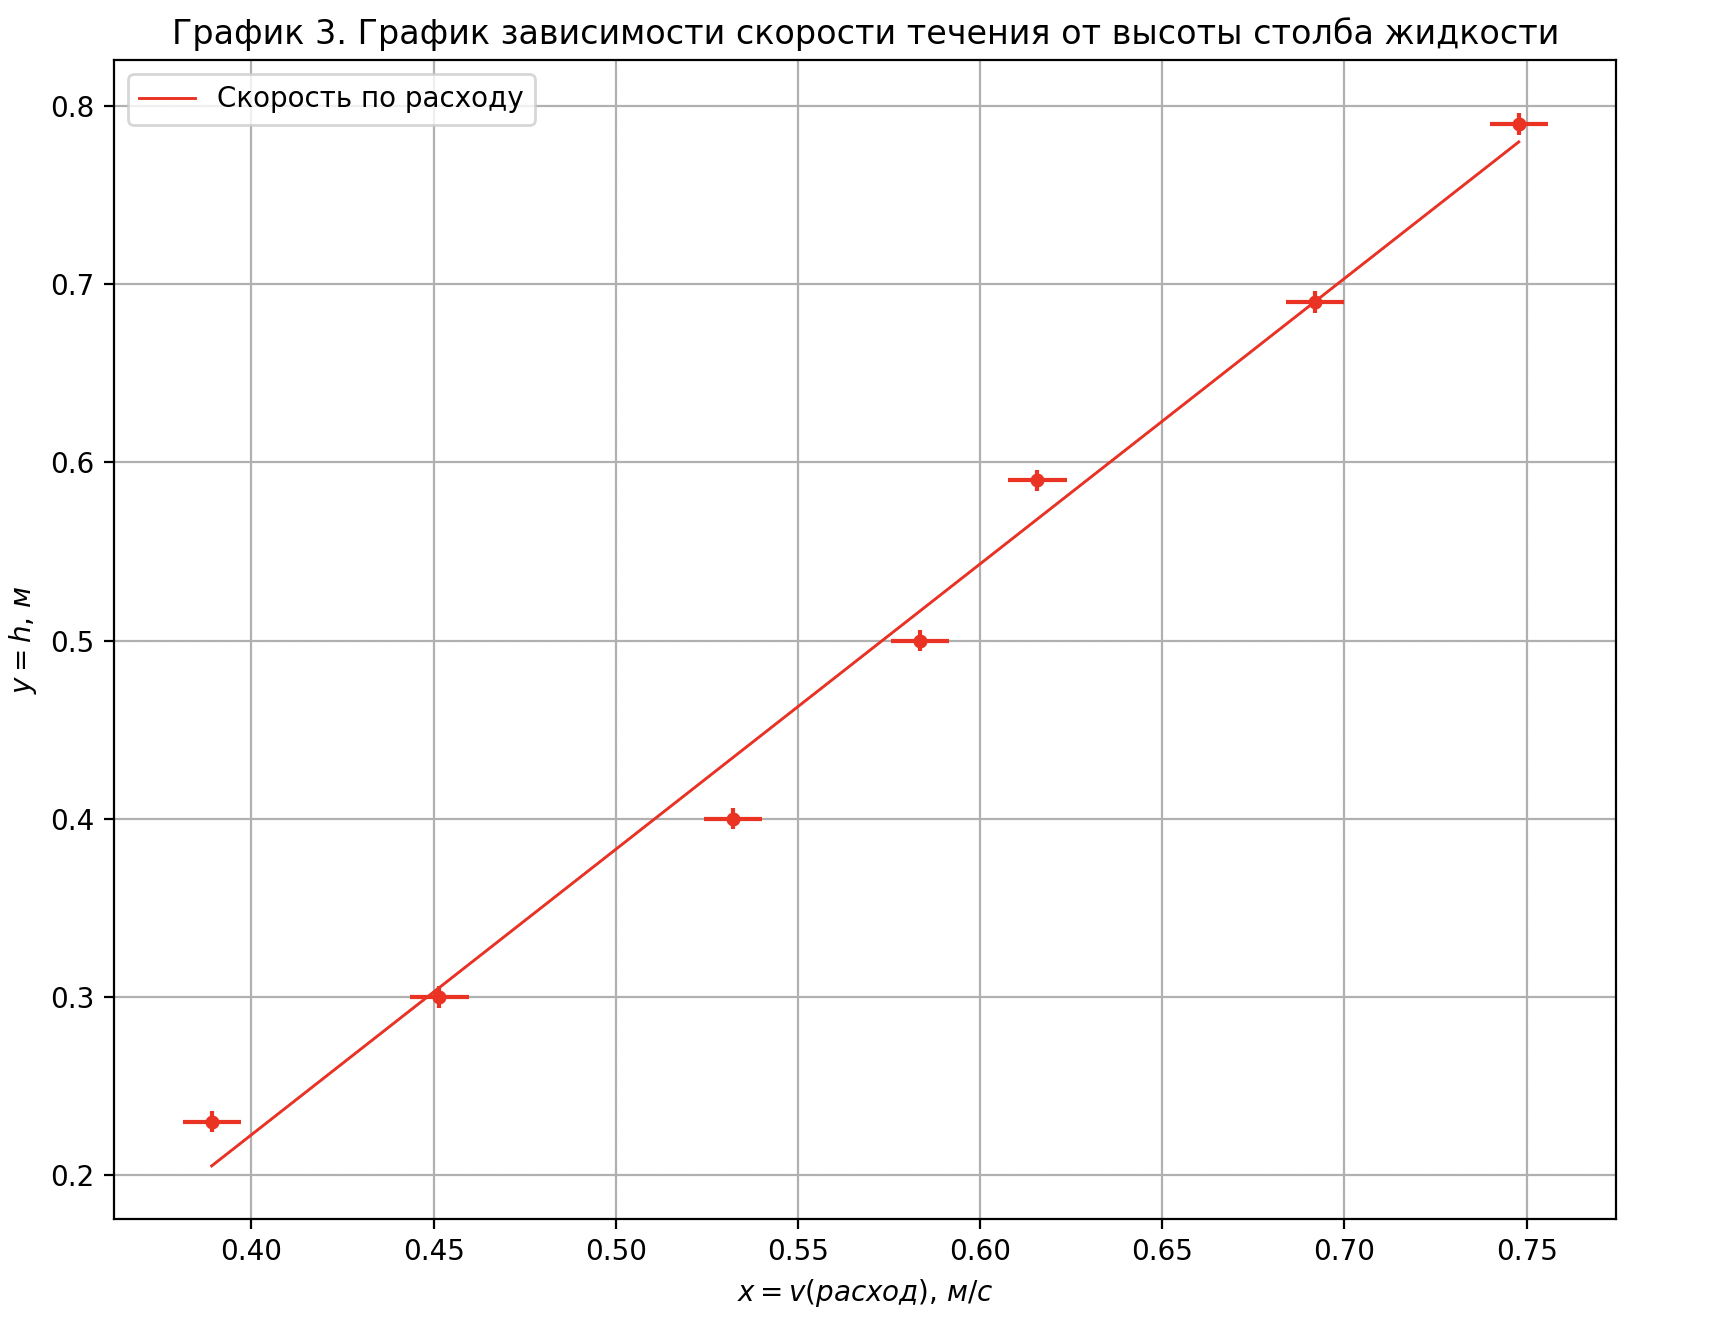
\includegraphics[width=18cm]{Snimok_Ekrana_2023-06-11_V_20_28_12.png}
	\end{center}
	\caption{График зависимости скорости течения по расходу от высоты}
	\label{ust}
\end{figure}

Вычислим значение числа Рейнольдса для точки, в которой теряется линейный характер графика: при $v = 0.39$ м/с определим число Рейнольдса по формуле $Re = \frac{v_pR\rho}{\eta} = 1950 \pm 60$(Вязкость воды $\eta = 0.001 Па \cdot c$.) В справочниках указано, что в трубе круглого сечения переход течения воды при комнатной температуре из ламинарного в турбулентный режим происходит при $Re \approx 1800$.
Теоретическая скорость, когда течение станет турбулентным: $v = 0.36$м/с


\subsection*{Выводы}
В ходе работы было исследовано течение жидкости в цилиндрической трубе, изучен принцип работы расходомеров Вентури и Пито, исследован стационарный режимы течения жидкости.Использование уравнения Торричелли для расчёта столба жидкости по скорости её течения неуместна по причине того, что рассматривается реальная, а не идеальная жидкость.Из-за турбулентного характера движения жидкости в резервуаре при его заполнении мы не можем применять формулы для ламинарного етчения жидкости.Были исследованы расходомеры Пито и Вентури, определены поправки для более точного расчёта скорости воды по их показаниям. Выяснилось, что наиболее точным является расходомер Вентури. Расходомер Пито показывает повышенное значение скорости, так как его трубка расположена в центре потока.

\end{document}